\subsection{比赛视频证据与源码对应}\label{sec:video-evidence}
\subsubsection{材料范围与取证方法}
本次新增原始材料为“比赛视频\texttt{.mp4}”，文件名由提供者给定；其视频流包含6830帧，分辨率960$\times$544，名义帧率约29\,fps，总时长235.52\,s。本文时间均为视频起点后的相对时间，不是 ROS 时间，也不是任务起止计时。原片在机器人、操作者电脑与其他现场位置间多次切换，不能以视频总时长计算比赛耗时。截图从原片解码保存，仅裁去无关边缘以突出机器人和屏幕，原始帧完整保留，不生成或补绘实验内容；帧号、时间及原文件 SHA-256 摘要记录于\code{data/video_evidence.json}。

由于提供者无法确认车辆与方式编号的对应关系，本文使用“近端跟随车”和“后续车辆”作为画面描述。带有某种标签的外观并不唯一确定 ROS 节点或输入源；图像中的排队顺序也不等于\code{tb1}至\code{tb4}命名空间顺序。因此，下面的图像用于验证现场现象，算法归因以代码和运行配置为准。

\subsubsection{起始准备与持物状态}
图\ref{fig:video-carry}将准备阶段与后续抱物阶段并列，目的是区分“机器人出现在场内”和“已经处于持物运行状态”。76\,s画面中物块位于机器人身前的低位，人员仍在邻近底盘处操作；133\,s画面中可见物块抬起，TonyPi 与移动底盘处于同一围挡通道。两帧不覆盖抓取全动作，不能由此认定抓取期间完全没有人工干预。
\begin{figure}[H]\centering
\begin{subfigure}{.485\linewidth}\centering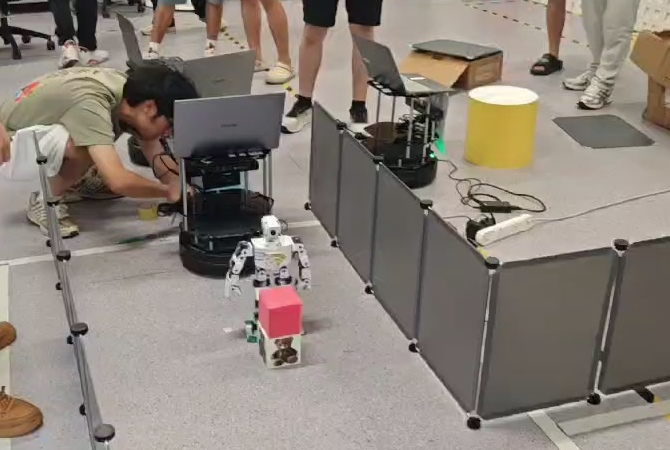
\includegraphics[width=\linewidth]{figures/video/competition_076s_focus.jpg}\caption{V076：76\,s，起始准备与近端底盘}\end{subfigure}\hfill
\begin{subfigure}{.485\linewidth}\centering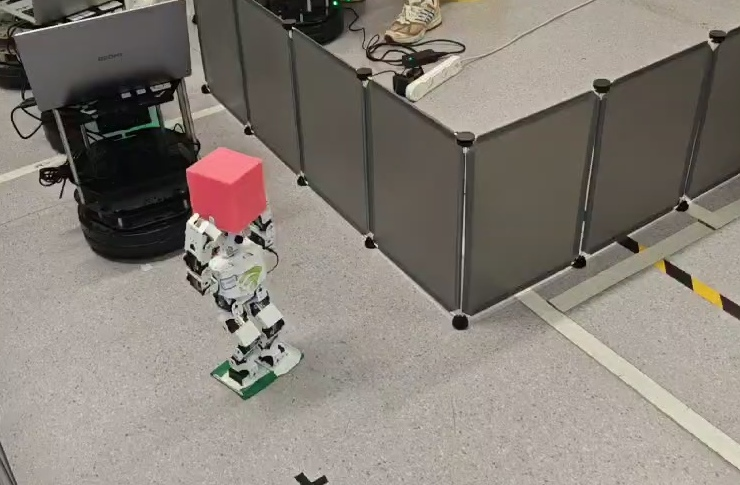
\includegraphics[width=\linewidth]{figures/video/competition_133s_focus.jpg}\caption{V133：133\,s，物块抬起后的现场}\end{subfigure}
\caption{准备与抱物画面对照，均为原始视频帧。}\label{fig:video-carry}
\end{figure}
这组对照支持在报告中加入真实持物场景，但抓取可靠性仍不能只用一帧终态评价。源码的抓取动作结束与物块实际被可靠夹持是两个事实：前者可由程序日志确认，后者需要动作全过程和物块状态的连续观察。人员出现在机器人附近也只按画面记录，不据此推断其是否操作遥控。

\subsubsection{通道推进与遮挡约束}
图\ref{fig:video-progress}选择165\,s和196\,s两个视角，用于展示抱物状态下的人形机器人、近端移动底盘及折线围挡的相对关系。与前一组准备图相比，这一组重点在于运行空间：通道限制横向余量，转角使后续车辆与目标间的直接视线变化，拍摄视角也随之改变。
\begin{figure}[H]\centering
\begin{subfigure}{.485\linewidth}\centering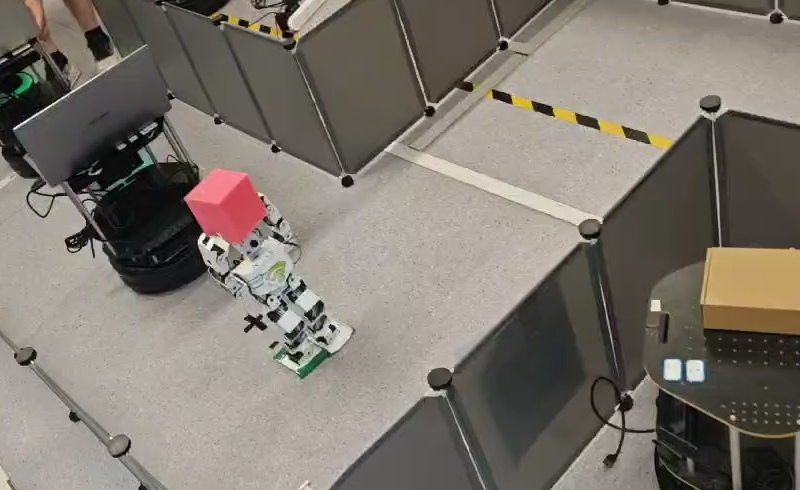
\includegraphics[width=\linewidth]{figures/video/competition_165s_focus.jpg}\caption{V165：165\,s，围挡内的抱物运行画面}\end{subfigure}\hfill
\begin{subfigure}{.485\linewidth}\centering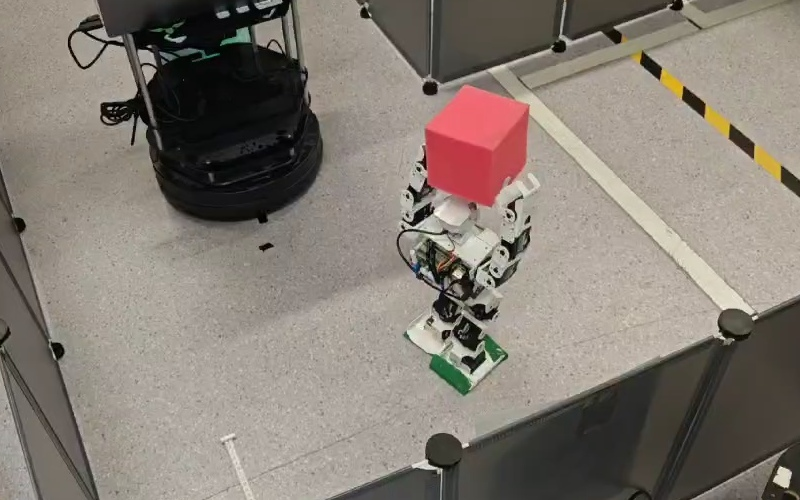
\includegraphics[width=\linewidth]{figures/video/competition_196s_focus.jpg}\caption{V196：196\,s，后续通道位置}\end{subfigure}
\caption{通道内的异构平台运行场景；不据透视图估计米制间距。}\label{fig:video-progress}
\end{figure}
两帧说明真实围挡与机器人共同构成了遮挡和通行约束，但镜头移动使像素位移无法直接换算机器人路程。没有平面标定、外部位姿或可复核尺度时，本文不从画面测量0.9\,m跟随间距，也不计算转向角误差。近端底盘与 TonyPi 同场出现不等于已证明其使用方式二或方式四，更不能由这些时刻的画面推出四车始终同步。

\subsubsection{标记识别与状态转换的调试证据}
184\,s处镜头转向操作电脑，画面同时包含相机标记识别窗口与路线终端日志。图\ref{fig:video-debug}的用途与前两组实景不同：它提供视觉目标与状态机分支同时存在的现场记录，可与\code{marker_route.py}中的路线观测、单次转向和\code{corner}搜索分支对应。
\begin{figure}[H]\centering
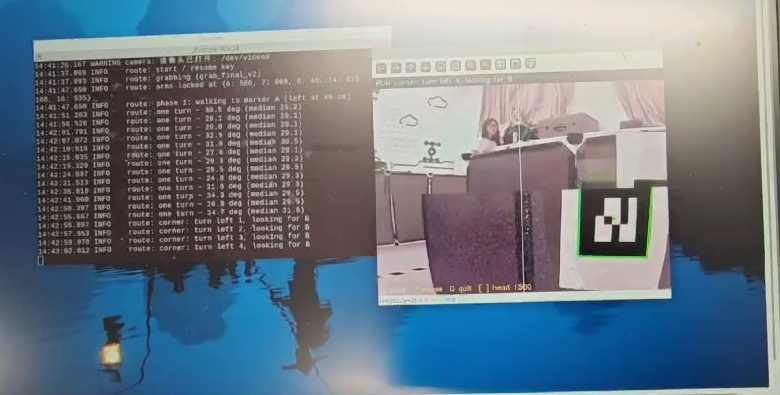
\includegraphics[width=.87\linewidth,height=.29\textheight,keepaspectratio]{figures/video/competition_184s_focus.jpg}
\caption{V184：184\,s，电脑上的标记检测窗口与路线调试日志。保留屏幕反光与拍摄透视，不把不可读字符补写成测量值。}\label{fig:video-debug}
\end{figure}
画面可辨认到标记检测框及寻找下一标记的路线日志，与“到达当前目标后进入转角搜索”的控制结构相符。这是源码状态转换具有现场调试对应物的证据，不能替代原始\code{decisions.csv}，也不据屏摄数字计算距离误差或控制周期。电脑显示的系统日期、终端时刻与视频相对时间尚未同步，本文只使用后者定位证据。

\subsubsection{后段画面与完成条件的界限}
图\ref{fig:video-late}取218\,s处后段画面，目的是记录视频后段仍可见的人形持物状态和邻近底盘位置。该图不能标为“终点放置成功”：当前视角没有完整展示物块由手臂释放、稳定留在目标区域以及末车持续停稳的全过程。
因此，本次可将证据等级从“仅有源码和照片”更新为“有现场视频支持的部分运行过程”，同时保留完整任务成功率、末车到达率和终点保持时间的测量空缺。未观察到某事件不等于事件未发生；本文只说明提交材料未形成足够的完整验收证据，不据此否定实验的其他未拍摄阶段。
\begin{figure}[H]\centering
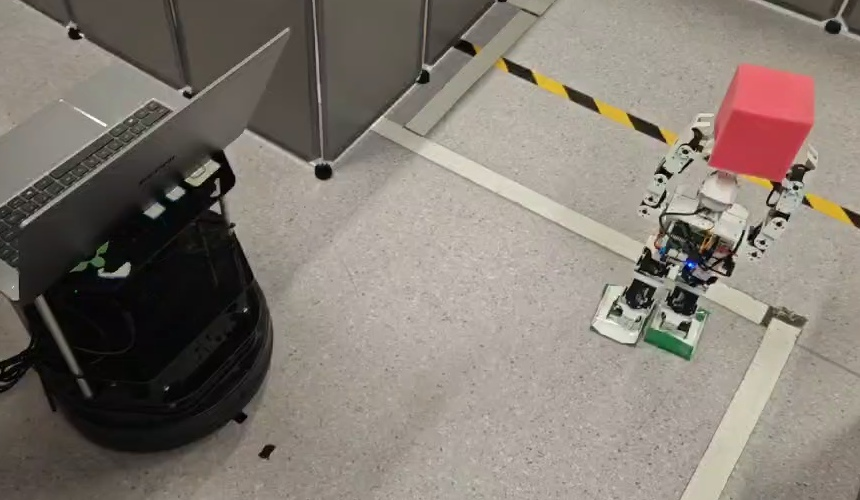
\includegraphics[width=.74\linewidth,height=.27\textheight,keepaspectratio]{figures/video/competition_218s_focus.jpg}
\caption{V218：218\,s，视频后段的机器人与物块状态。该帧不构成终点放置或末车停靠验收。}\label{fig:video-late}
\end{figure}
该帧保留的是这一时刻的可见物体与机器人位置。终点验收还需在同一连续时间段内确认释放、物块稳定放置、机器人进入规定区域及末车保持停止，不能由单帧外观代替。

\subsubsection{证据归档及后续补充方式}
下表把已经获得的材料与仍需补齐的内容分开，使后续补充有明确对象。完整视频不重复装入 Overleaf ZIP；项目中保留被实际引用的原始帧和可复核索引，原片继续使用本地原路径归档。
\begin{table}[H]\centering\small
\caption{视频与代码共同支持的结论及剩余证据}
\begin{tabularx}{\linewidth}{p{30mm}XX}\toprule
问题 & 本次已获得 & 仍需材料\\\midrule
TonyPi 抱物运行 & V133、V165、V196等现场帧 & 全过程日志及掉落、碰撞核验\\
标记状态机 & V184检测窗口和转角搜索日志；对应代码 & 原始决策日志与同步时间基准\\
底盘与队列 & 多车布置及近端底盘同场画面 & 车辆编号、启动参数、话题连接\\
方式四控制机制 & 前车位姿模式、轨迹与守卫代码 & 对应实车日志和输入实际频率\\
终点完整验收 & 目前后段帧不能闭合放置与停稳链 & 放置全过程、末车停靠、全队结果\\\bottomrule
\end{tabularx}\end{table}
后续可以直接提供起点至终点的连续录像或运行日志目录，无需先整理成报告。若能再提供每台车对应的命名空间和启动命令，便可把“近端跟随车”替换为实际方式编号，并把视频事件与位姿、许可和速度时间线对齐。在这些信息缺失时，保持画面事实与算法机制分别论证。
